\section{Usmereni aciklični graf}

Usmereni aciklični graf predstavlja strukturu podataka koja se sastoji od skupa čvorova povezanih ivicama, pri čemu te veze imaju smer i ne formiraju nikakve cikluse. U ovoj strukturi čvorovi označavaju entitete poput podataka ili objekata, dok veze predstavljaju relacije između njih~\cite{ibm DAG}.

Na slici~\ref{fig:dag slika} je prikazan primer usmerenog acikličnog grafa.

% \begin{figure}[h]
%     \centering
%     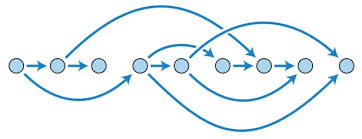
\includegraphics[width=0.6\textwidth]{slike/dag_blue.jpeg}
%     \caption{Primer usmerenog acikličnog grafa}
%     \label{fig:dag slika}
% \end{figure}

\begin{figure}[h]
    \centering
    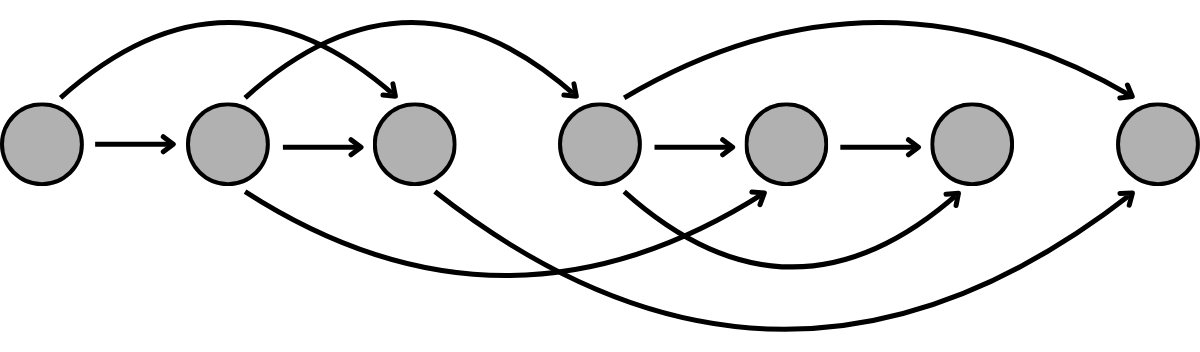
\includegraphics[width=0.6\textwidth]{slike/my_dag.png}
    \caption{Primer usmerenog acikličnog grafa}
    \label{fig:dag slika}
\end{figure}


Osnovne karakteristike DAG-ova su njihova usmerenost i acikličnost. Usmerenost podrazumeva da svaka veza između dva čvora ima definisan smer, čime se omogućava određivanje parcijalnog redosleda elemenata. Acikličnost znači da, ukoliko se prati smer usmerenih veza, nemoguće je doći do početnog čvora od kojeg se krenulo~\cite{ibm DAG}.

Kao koncept iz teorije grafova, DAG strukture se široko koriste u različitim oblastima računarskih nauka i inženjerstva upravo zato što dozvoljavaju da se identifikuju i obrađuju složene zavisnosti bez rizika od beskonačnih petlji ili konflikata među operacijama. Neke od njihovih primena su rešavanje problema raspoređivanja zadataka i planiranja, upravljanje lancima snabdevanja, a najčešće se koriste za obradu tokova podataka~\cite{datacamp DAG}.

Ključna prednost usmerenog acikličnog grafa u odnosu na linearnu strukturu jeste upravo njegova sposobnost da omogući paralelnu obradu informacija i eliminaciju nepotrebnih čekanja, što može imati veliki značaj u okruženjima gde je efikasnost obrade kritična~\cite{datacamp DAG}. Upravo ove osobine čine DAG posebno interesantnim za primenu u distribuiranim knjigama, gde je fleksibilnost organizacije podataka i efikasno rešavanje zavisnosti između transakcija ključ za performanse i skalabilnost sistema.

% Kako bi se razumeo pojam usmerenog acikličnog grafa, važno je opisati ključne koncepte koji ga opisuju. U računarskim naukama, graf predstavlja nelinearnu strukturu podataka koja se sastoji od čvorova i ivica. Čvorovi predstavljaju određene entitete, dok ivice reprezentuju vezu ili relaciju između njih~\cite{datacamp DAG}.

% Kod usmerenih grafova, ivice sadrže smer, reprezentujući time jednosmernu vezu između čvorova. Usmereni aciklični grafovi ne dozvoljavaju ciklične relacije između čvorova.

% Na slici ... je prikazana struktura usmerenog acikličnog grafa.